\documentclass[12pt]{article}
\usepackage[a4paper, margin=3cm]{geometry}
\usepackage{graphicx}
\usepackage{wrapfig}
\usepackage{subfig}
\usepackage{csquotes}
\usepackage{booktabs}
\usepackage{tabularx}

\usepackage[dvipsnames]{xcolor} % Color names
\definecolor{accent}{HTML}{008080}
\usepackage{hyperref}
\hypersetup{
    colorlinks=true,
    linkcolor=accent,
    anchorcolor=black,
    citecolor=accent,
    filecolor=black,
    menucolor=black,
    runcolor=black,
    urlcolor=accent}
\hypersetup{breaklinks=true}
\usepackage{url}
\usepackage{authblk}
\usepackage{soul} % strikethrough \st{}; highlight \hl{}
\usepackage{bidipoem}
\usepackage[final]{microtype}



% Bibliography information processing
\usepackage[
    backend=biber,
    style=apa,
    autocite=inline,
    sorting=nyt,
    sortcites=true,
    backref=false,
    backrefstyle=three,
    abbreviate=true,
    block=space,
]{biblatex}
% \DefineBibliographyStrings{american}{
%     backrefpage={Cited on p.},
%     backrefpages={Cited on pp.}
% }
\apptocmd{\sloppy}{\hbadness 10000\relax}{}{}
\appto{\bibsetup}{\sloppy}
\DeclareFieldFormat{apacase}{#1} % Title casing in APA
% \AtBeginBibliography{\small} % Can make the font in bibliography smaller

\addbibresource{../static/bibliography/parti.bib} %



% Languages, scripts, and fonts

% Font packages
\usepackage{libertine} % Latin, Greek, Cyrillic, Hebrew

% Fontspec
\usepackage{fontspec}
\defaultfontfeatures{Ligatures={TeX}}

% % Language settings
\usepackage[main=english, bidi=basic]{babel}

% Automatic typesetting of certain writing systems
\babelprovide[import=ar, onchar=ids fonts]{arabic}
% \babelprovide[import=he, onchar=ids fonts]{hebrew}
\babelprovide[import=sa-Deva, onchar=ids fonts]{sanskrit-devanagari}

% Define fonts (https://tug.org/FontCatalogue/)
% \babelfont{rm}{Linux Libertine}
% \babelfont{sf}{Linux Biolinum}
% \babelfont{tt}{Inconsolata}

\babelfont[*arabic]{rm}{Noto Naskh Arabic} % Amiri
% \babelfont[*hebrew]{rm}{Linux Libertine} % Noto Serif Hebrew
\babelfont[*devanagari]{rm}[Renderer=Harfbuzz]{Noto Serif Devanagari} 
% % Settigs: Scale=MatchUppercase; Scale=MatchLowercase; Scale=1.0; Language=Default

% East Asian scripts
% \usepackage{kotex} % Support for KR, JP, some TC (not SC).
% \setmainhangulfont{Noto Serif CJK KR} % Only on Overleaf
% \setmainhangulfont[
    % Path=./fonts/,
    % Extension = .otf,
    % UprightFont=*-Medium,
    % BoldFont=*-Bold
    % ]{NotoSerifKR}

\newfontfamily{\traditionalchinesefont}[
    Path=./fonts/,
    Extension = .otf,
    UprightFont=*-Medium,
    BoldFont=*-Bold
    ]{NotoSerifTC}

% \newfontfamily{\simplifiedchinesefont}[
%     Path=./fonts/,
%     Extension = .otf,
%     UprightFont=*-Medium,
%     BoldFont=*-Bold,
%     ]{NotoSerifSC}

\newfontfamily{\khmerfont}[
    Path=./fonts/,
    Extension = .otf,
    UprightFont=*-Regular,
    % BoldFont=*-Bold,
    ]{NotoSerifKhmer}

\newfontfamily{\javanesefont}[
    Path=./fonts/,
    Extension = .otf,
    UprightFont=*-Regular,
    % BoldFont=*-Bold,
    ]{NotoSansJavanese}

% Other scripts
\newfontfamily{\tibetanfont}[Script=Tibetan]{Noto Serif Tibetan}

% Commands to use scripts
\newcommand{\bo}[1]{\tibetanfont{#1}\rmfamily}
\newcommand{\tc}[1]{\traditionalchinesefont{#1}\rmfamily}
\newcommand{\km}[1]{\khmerfont{#1}\rmfamily}
\newcommand{\jv}[1]{\javanesefont{#1}\rmfamily}
% \newcommand{\zh}[1]{\simplifiedchinesefont{#1}\rmfamily}

% Keywords command
\providecommand{\keywords}[1]{\small\noindent\textbf{\textit{Keywords ---}}#1}

% ORCiD
\definecolor{orcid}{HTML}{A6CE39}
\usepackage{academicons}
\newcommand{\orcid}[1]{\href{https://orcid.org/#1}{\textcolor{orcid}{\aiOrcid}}}



\title{Cardamoms in China, and the etymology of \textit{dòukòu} `cardamom; nutmeg'}
\author[1]{{\small\orcid{0000-0003-2042-4655}}~Gábor Parti}
\author[2]{{\small\orcid{}}~Ian Joo}
\affil[1,2]{The Hong Kong Polytechnic University}
\affil[2]{Nagoya University of Commerce and Business}
\date{\small{February 2024}}

\begin{document}

\setlength{\tabcolsep}{2pt} % Change table padding

\maketitle

\begin{abstract}
    This paper aims to provide a new etymological explanation for the Chinese word \tc{豆蔻} \textit{dòukòu} `cardamom; nutmeg' and explore the potential trade-language origins of the term. We propose that this word is a borrowing that may have entered the Chinese lexicon via Southern Min, originating from an Indian Ocean trade-language used on the ancient Maritime Silk Road during the Tang era (618--907). Our findings suggests that \textit{dòukòu} entered the Chinese lexicon alongside the economic products it denotes, and underwent phono-semantic matching that obscured its foreign origin. We present our rationale in four main points, detailing our observations regarding 1) the earliest written records, 2) character composition, 3) available lexicographical data, and 4) an overview of regional \textit{Wanderwörter} (wandering loanwords) as evidence supporting our hypothesis. After uncovering the lexicogenesis of this word, we discuss the linguistic and historical plausibility of our claims, and explore potential candidate etymons, such as Prakrit and Arabic. Additionally, we also clarify the situation surrounding cardamoms from an Asian perspective, focusing on their identities, origins, and terminology in Chinese.

\end{abstract}

\noindent{\small\textbf{\textit{Keywords --- }} Cardamom, \tc{豆蔻}, Etymology, Trade-language, Chinese, Southern Min, Indian Ocean, Spice Trade}

\section*{Notes and todo list}

\begin{itemize}
    \item Text in \hl{highlight} needs to be checked; corrected; finalized.
    \item ?? indicates need for explanation; verification; citation.
\end{itemize}

\clearpage



\section{Introduction}

Cardamom is a popular spice with a history spanning thousands of years of culinary and medicinal use; the reader might recall its vibrant aroma. Less well-known is the fact however, that the name \textit{cardamom} can refer to multiple different kinds of fragrant fruits, besides the familiar green pods of the ``true cardamom''. Furthermore, delving deeper into the intricacies of cardamoms from an Asian perspective reveals a complex array of words and materials, as many prototypical cardamoms grown in various regions (e.g., Eastern Himalayas, Indochina, Yunnan, Java) are botanically distinct species, and their names and identities have become entangled along the paths of diffusion.

In this study, we examine the situation in Chinese, where the corresponding word is \tc{豆蔻} \textit{dòukòu} -- also referring to another important spice, nutmeg. Similarly to its equivalent in English, \textit{dòukòu} acts as an umbrella term that can refer to any of a number of cardamom-type fruits and other closely associated spices. Its precise meaning is defined by regional and dialectal actualities, and narrowed by modifiers.

The main objective of this paper is to offer a novel etymological explanation for the Chinese term \textit{dòukòu} `cardamom; nutmeg', and explore its potential trade-language origins. We posit that this term is a loanword that may have been incorporated into Chinese via Southern Min, originating from a yet unidentified Indian Ocean trade-language that was in use along the ancient Maritime Silk Road during the Tang dynasty (618--907) or earlier, when this term first appears in written records. Our research suggests that this word entered the Chinese lexicon alongside the economic products it denotes, and underwent phono-semantic matching that masks its foreign origin. 

We present our reasoning in four main points, outlining our observations on 1) the earliest written attestations, 2) character composition, 3) available lexicographical data, and 4) an overview of seemingly related regional \textit{Wanderwörter} (wandering loanwords) from the Indian Ocean world, as evidence supporting our hypothesis.

% Tamil?
% something about history?

% \textit{Dòukòu} first appears as \textit{báidòukòu} [white-cardamom] in a Tang-era miscellany called \textit{Youyang Zazu}, where it is reported to come from the land of \hl{Kakkola}, describing the white, round cardamoms of (\textit{Wurfbainia vera} or \textit{Wurfbainia compacta}) originally sourced either from Siam or Java. According to this 9th-century source, the spice is called \tc{多骨} \textit{duōgǔ}, and the perceived Middle Chinese pronunciation, /tɑ-kuət̚/ ??, makes possible for it to be a sinicized transcription of an \hl{Indo-Aryan} word, e.g., from Prakrit. On the other hand, the same does not apply for \tc{豆蔻} \textit{dòukòu}, whose Middle Chinese pronunciation would be /dəuH-həuH/ ??. 

% personal communication, August 17, 2022

% As an alternative, we propose that \textit{dòukòu} could be a loan via Southern Min. Based on Kwok's reconstruction of Proto-Southern-Min, the equivalent of \textit{dòukòu} would be /*tɑu-khɑu/ \parencite{kwok_2018_southern}, more similar to the Indic words in question. 

% This is historically plausible, given that Fujian was in direct contact with the maritime traders responsible for the bulk of the spice trade, and that Sanskrit was one of the main languages of the Srivijaya Empire encompassing Kakkola around this time. In this brief etymological study, we clear the air around cardamom nomenclature, and reveal a possible trace that Fujianese traders have left on modern Chinese. This is not only interesting in terms of food history, but also in terms of the linguistic history of Chinese, as few loanwords from Southern Min have made their way into Middle Chinese.

The paper also seeks to clarify the situation surrounding the multitude of cardamoms in Asia, focusing on their origins and terminologies within a Chinese context. As it was just mentioned above, the meaning of the word \textit{dòukòu} itself can be ambiguous, and has been so since its earliest emergence; it can refer to several different aromatic fruits and seeds. The identity of \textit{dòukòu} therefore is one of the central problems to be solved while tracing the word's history.

% ab ovo

In section \ref{sec:plants}, we begin with a brief introduction to what cardamoms are, identifying the relevant plants and their products used in the various regions of tropical and subtropical Asia, accompanied with their nomenclature in Chinese. This will establish a foundation for our linguistic inquiries that is based on geobotanical realities. Then, in section \ref{sec:etymology}, we present our etymological hypothesis, and discuss the evidence and reasoning behind it. Following the elucidation of the lexicogenesis of this term, we examine potential candidate etymons, such as Prakrit and Arabic, discuss the linguistic and historical plausibility of our claims, and acknowledge the limitations.

\section{The cardamom conondrum}\label{sec:plants}

\subsection{What is cardamom?}


What people mean by the name \textit{cardamom} depends on who we ask, where we are, and in what language we are operating -- for the word \textit{cardamom} and its translations can denote multiple different spices. In all cases, this name will refer to an aromatic plant yielding a culinary and medicinal spice, and in all likelihood, most readers will think of the green, dried fruits of a tropical plant known as \textit{Elettaria cardamomum} (L.) Maton\footnote{Binomial nomenclature: \textit{Elettaria} marks the genus name (capitalized, can be abbreviated); \textit{cardamomum} is the ``specific epithet'', followed by the authority who published and described the plant (optional). These three elements can identify a plant beyond doubt. In this case William George Maton reclassified and thus renamed the previous taxon by Linnaeus (hence the L.), which was \textit{Amomum cardamomum} L., now considered a (superseded) ``synonym''.} seen in Figure \ref{fig:cardamom}.

% \begin{figure}[h]
%     \centering
%     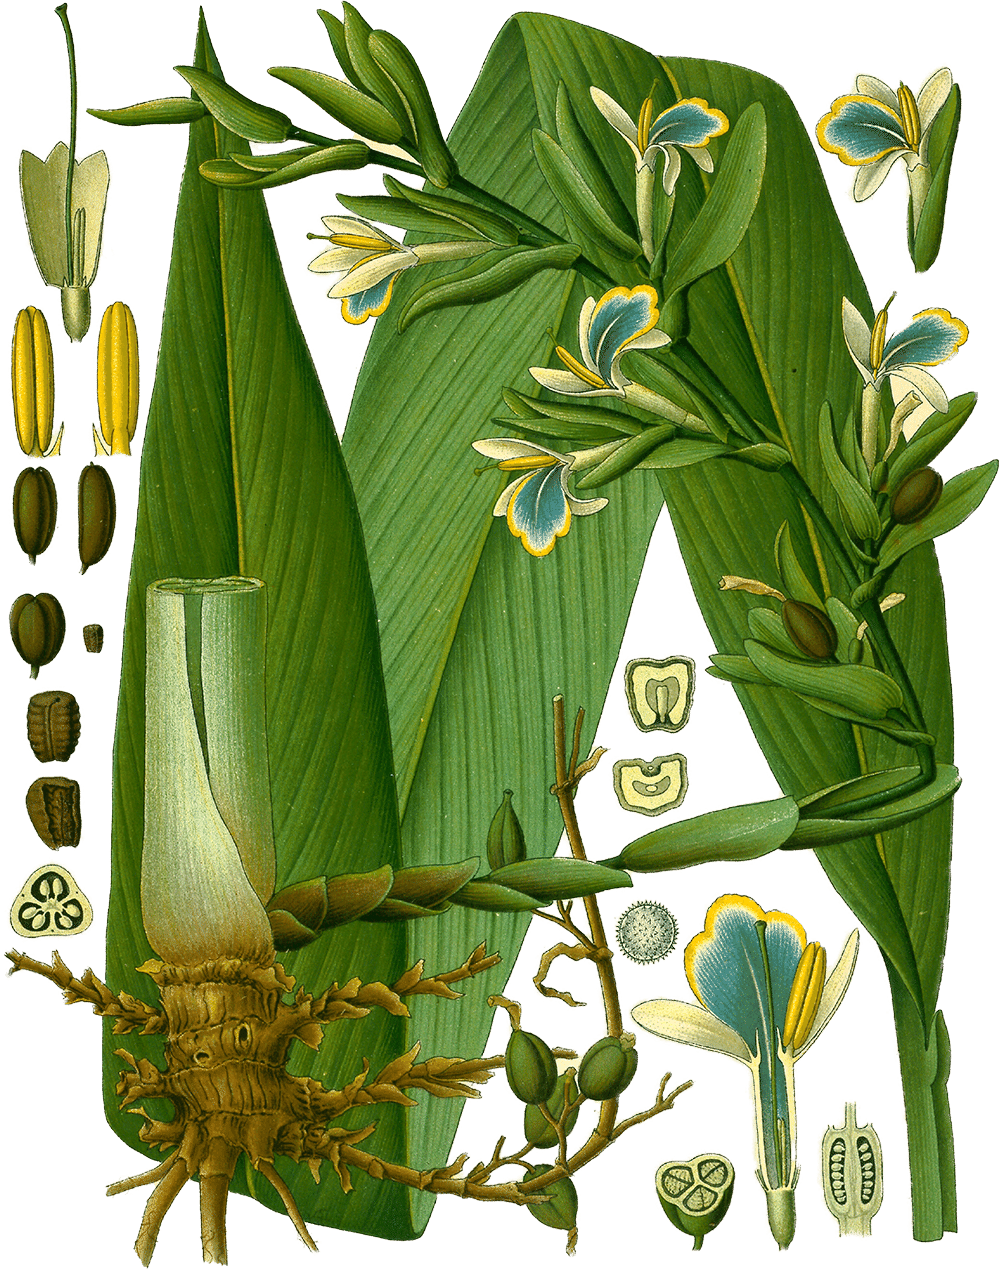
\includegraphics[width=0.45\textwidth]{imgs/cardamom.png}
%     \caption{\textit{Elettaria cardamomum} in \textit{Köhler's Medizinal Pflanzen} \pvolcite[]{2}[186]{koehler_1887_koehler}}
%     \label{fig:cardamom}
% \end{figure}

\begin{wrapfigure}{r}{0.5\textwidth}
    \centering
    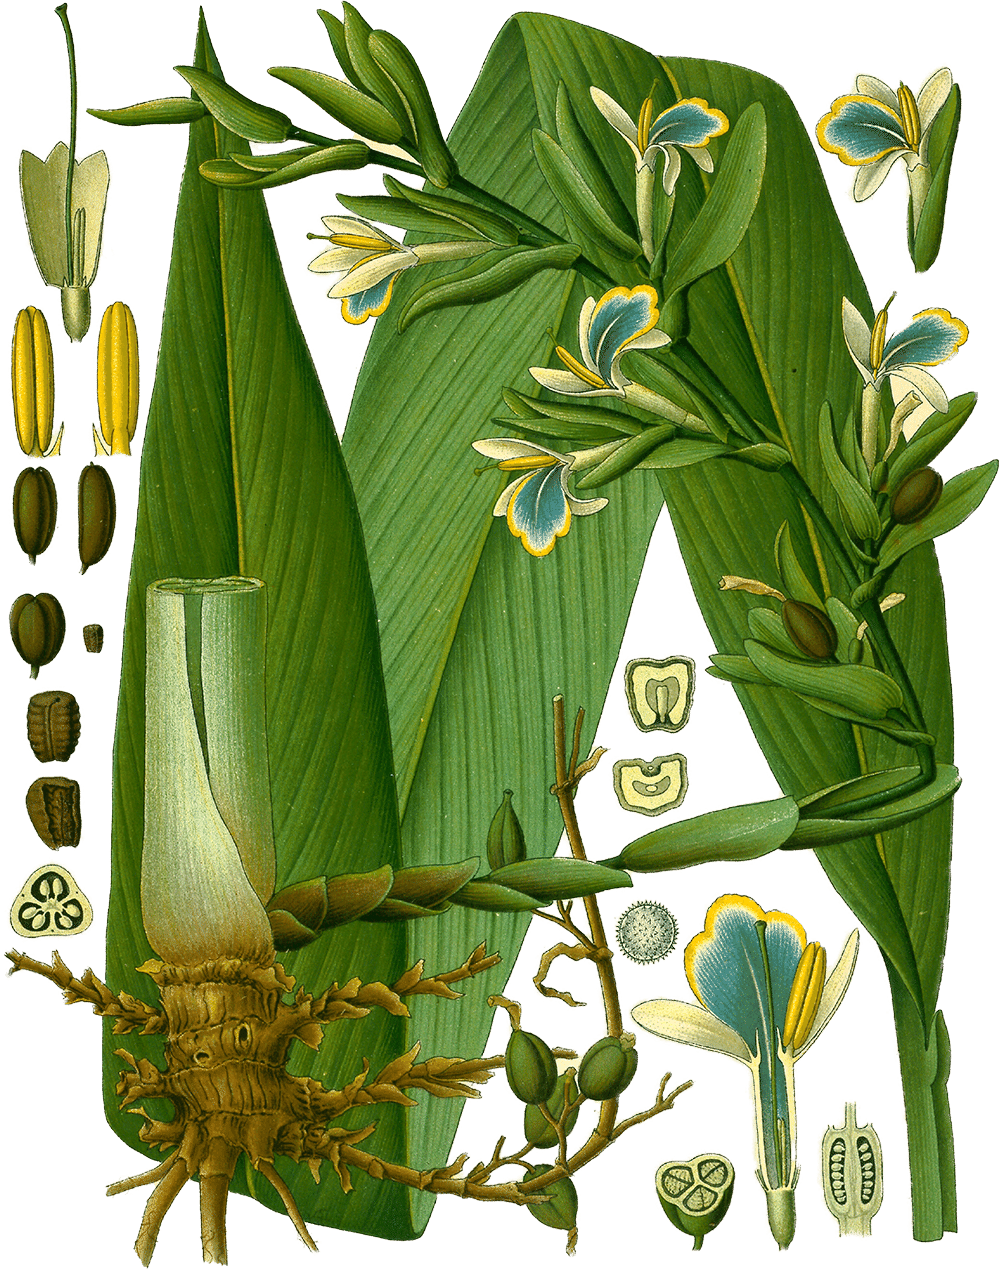
\includegraphics[width=0.5\textwidth]{imgs/cardamom.png}
    \caption{\textit{Elettaria cardamomum} in \textit{Köhler's Medizinal Pflanzen} \pvolcite[]{2}[186]{koehler_1887_koehler}}
    \label{fig:cardamom}
\end{wrapfigure}

% ഏലത്തരി elattari in Malayalam, where the genus name is from (1811)

In Europe, the Middle East, India, and many other parts of the world, \textit{cardamom} typically refers to the seed pods of \textit{E. cardamomum},\footnote{\textit{Elettaria cardamomum} in Plants of the World Online \parencite{powo}: \url{https://powo.science.kew.org/taxon/796556-1}} which is an aromatic flowering plant in the ginger family (\textit{Zingiberaceae}). It is native to India's Western Ghats, the mountain range streching along the Malabar coast of Kerala. This is the same region where black pepper hails from, and in an Indian context they are often called ``the king and queen of spices'' -- cardamom being the queen \parencite{nair_2011_agronomy}. 

It is a well-known culinary spice with a long history of commerce, also used in the infusion of beverages, and perfumery. Think of Indian cuisine, Arabic coffee, Egyptian perfumes, etc. Cardamom has been in use in India since the Vedic period and was traded to and through Mesopotamia since the Bronze Age \parencite{ravindran_2002_cardamom}. In Europe, cardamom has been known since antiquity and was used as medicine. Greek physicians, such as Dioscorides and Galen have documented its healing properties, in some cases even correctly identifying India as its place of origin \parencites{parry_1969_spices}{anderson_2023_history}. Historiographers Theophrastus and Pliny (the Elder) described two types of cardamom: the superior καρδάμωμον \textit{kardámōmon} (\textit{E. cardamomum}) and the inferior ἄμωμον \textit{ámōmon} we now mostly call ``black cardamom'' (\textit{Amomum subulatum}) \parencite{prance_2005_cultural}, the latter of which has since lost its prevalence in Europe, but still obtainable from Indian grocers. During the Middle Ages, cardamom was traded in the Mediterranean primarily by Arab merchants to Venice, a monopoly broken by the Portuguese in the 16\textsuperscript{th} century, who established direct trade with the Malabar coast \parencite{cumo_2013_encyclopedia}. In his 1596 \textit{Itinerario}, Dutchman Linschoten reported ``lesser'' and ``greater'' cardamoms being used in southern India, corresponding to the smaller green cardamoms, and the larger black cardamoms mentioned above \parencite{nair_2020_geography}. These two are the main cardamoms of commerce today, and the only ones that are widely known in the West.

The green pods are still valuable today, it is the 3\textsuperscript{rd} most expensive spice after saffron and vanilla, due to its labor-intensive harvest. It is also known as \textit{green cardamom} and \textit{true cardamom}. From now on, we will refer to the fruits of \textit{E. cardamomum} as \textit{green cardamom} to avoid confusion.

% In China, cardamoms are exotic or semi exotic, Chinese sources feature significant trade in cardamoms during the Song dynasty (960--1279) \parencite{prance_2005_cultural}.

\subsection{False cardamoms}

Now, the name \textit{true cardamom} implies the existence of ``false'' ones, which is not so unusual in English spice nomenclature; it can happen for two reasons. First, the term \textit{false} and its synonyms are typically used to designate alternative economic products (cf. \textit{false peppers}). Second, they hint at practices of adulteration (cf. \textit{bastard saffron}). As one of the strategies employed to distinguish spices is by using a marker of authenticity, words, such as \textit{true, real, false, fake, bastard} can occur in vernacular names. In our case, the former holds true: there are at least a dozen other spice-bearing aromatic plants in the ginger family referred to as \textit{cardamoms}, two of which we have already mentioned. Until very recently, almost all cardamom-like plants were neatly sorted into two genera: the genus \textit{Amomum} with a native range spanning from South to Southeast Asia, and the genus \textit{Aframomum} distributed in Africa. Today, many of them boast with new and revised scientific names, which can make their discussion quite overwhelming.\footnote{Modern taxonomic classification of plants started with \textcite{linnaeus_1758_systema}, but it is still developing to this day -- English botanist Burkill have already lamented on the ``unwelcome'' renaming of some cardamom species almost a hundred years ago \parencite[see][]{burkill_1930_cardamoms}.}

So, why are these other spices being called \textit{cardamoms} as well? In short, these plants and their products are named so because of their physical, chemical, and functional similarities to a prototype spice, especially in one distinct feature: they are all aromatic seed pods containing small seeds. The compact fruits' shared morphology is distinctivie enough to warrant association with an already known item, which influences the naming of newly acquired and encountered spices. In a western context, the prototype spice is the green cardamom we know (\textit{E. cardamomum}), hence the name \textit{true cardamom}. We take the idea of a ``prototype spice'' from the prototype theory in cognitive science, as this seems to illuminate best the categorization and naming practices of new spices during acculturation \parencite[see][]{parti_2023_mapping}.

To clarify, false cardamoms are not fake. What is considered ``false'' is determined by the predominant prototype spice in a given culture (whether it is indigenous to the region, or the first of its kind encountered), and the perceived value of the spice affected by notions of quality and scarcity. For instance, Ceylon cinnamon from Sri Lanka has historically been regarded as superior to cassia or Chinese cinnamon, leading to the existence of names such as \textit{true cinnamon} (even dictating the scientific name, \textit{Cinnamomum verum}, meaning `true cinnamon' in Latin) and \textit{bastard cinnamon}.



\begin{figure}[h]
	\vspace{-2ex}
	\centering
	\subfloat{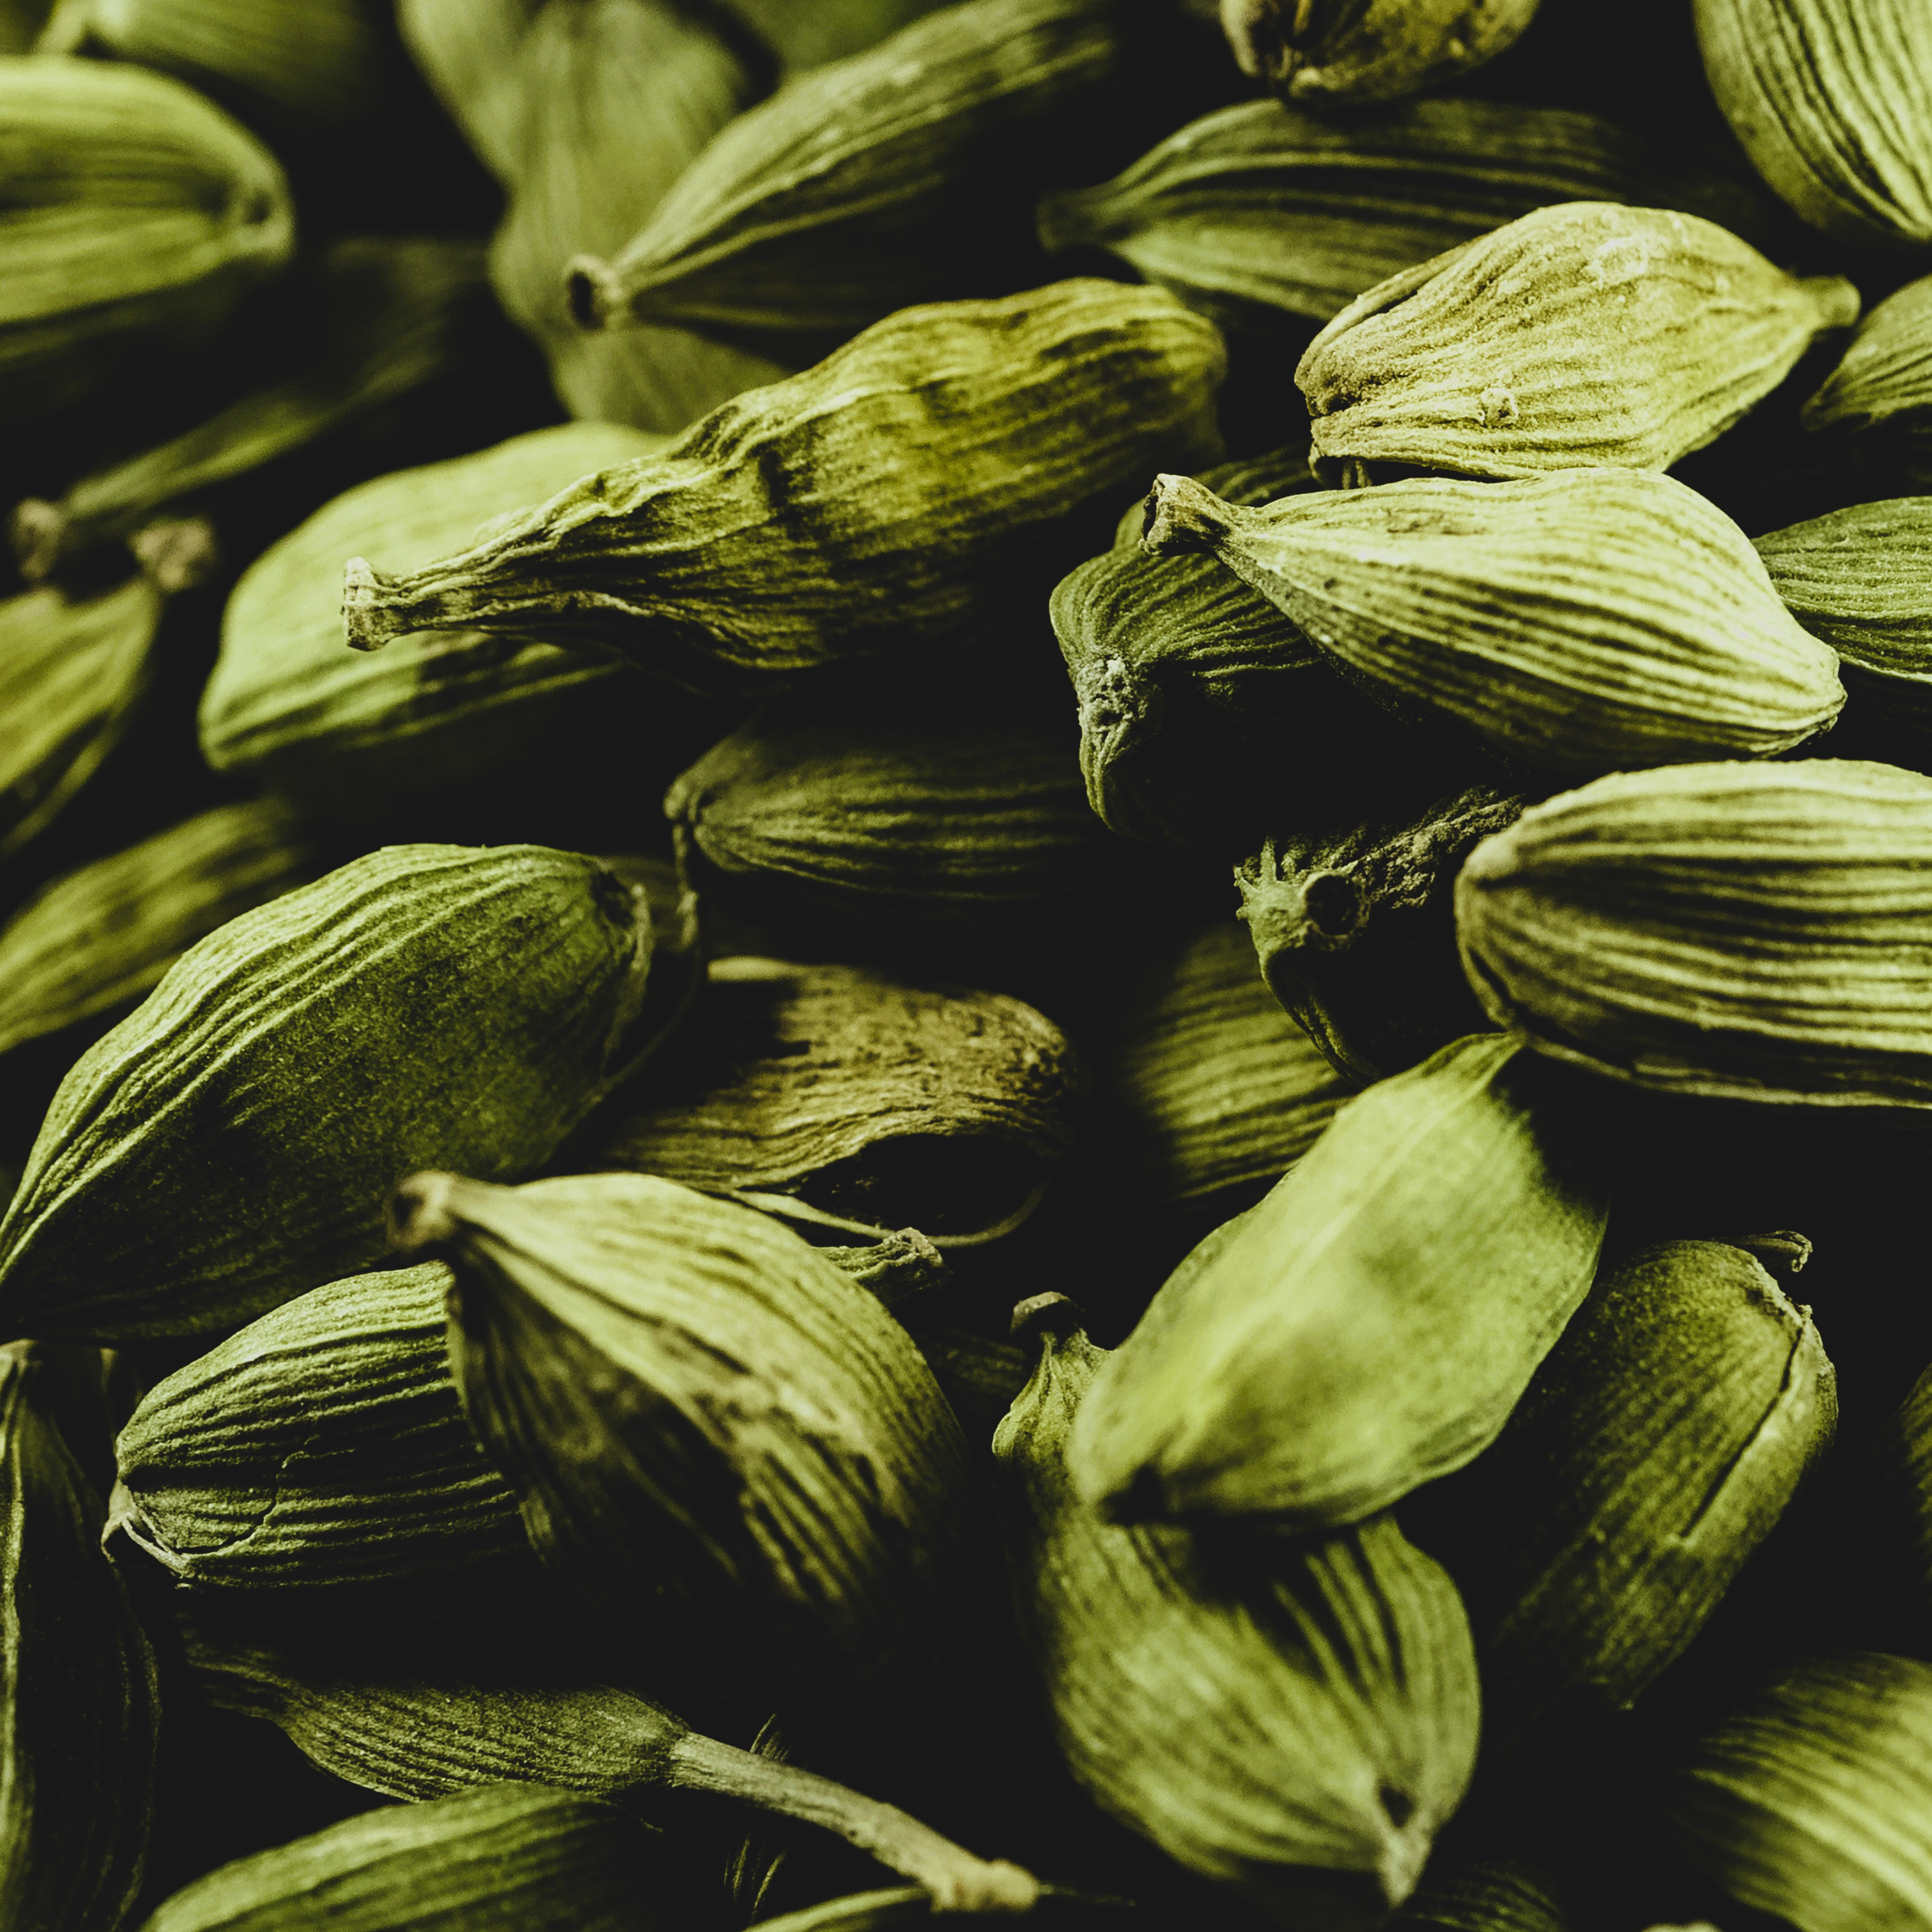
\includegraphics[width=0.23\linewidth]{imgs/green_cardamom.png}}
	\hfill
	\subfloat{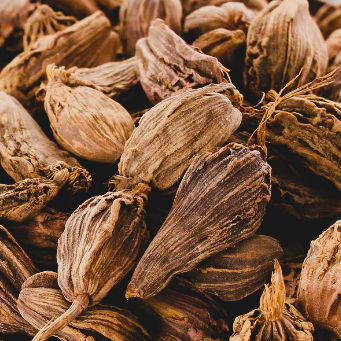
\includegraphics[width=0.23\linewidth]{imgs/black_cardamom.png}}
	\hfill
	\subfloat{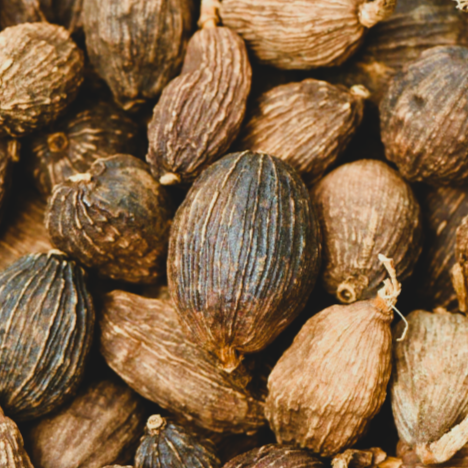
\includegraphics[width=0.23\linewidth]{imgs/tsaoko.png}}
	\hfill
	\subfloat{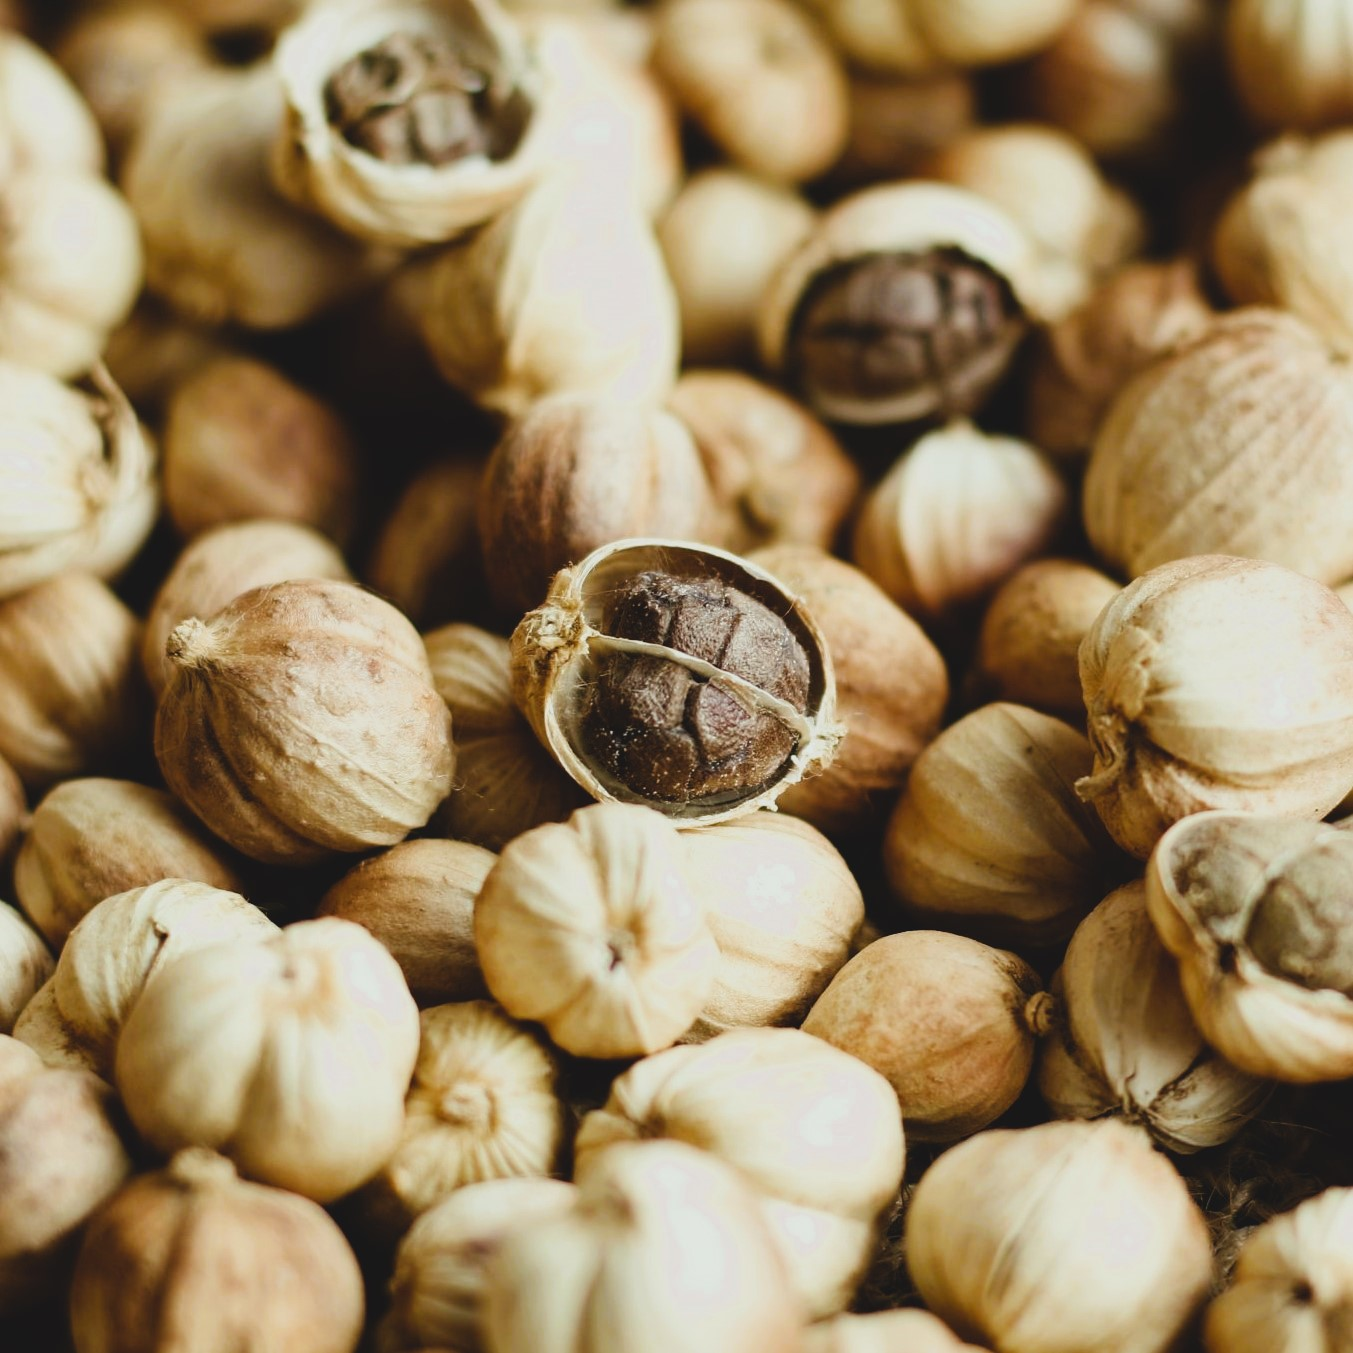
\includegraphics[width=0.23\linewidth]{imgs/white_cardamom.png}}
	\caption{From left to right: green cardamoms (\textit{Elettaria cardamomum}), black cardamoms (\textit{Amomum subulatum}), tsaoko cardamoms (\textit{Amomum tsao-ko}), and round cardamoms (\textit{Wurfbania compacta}). Photo: \href{https://www.pexels.com/photo/pile-of-green-cardamoms-6086300/}{Eva Bronzini}, \href{https://www.naturalplusgreen.com}{NPG}, \href{https://www.naturalplusgreen.com}{NPG}, \href{https://nai4trade.com/spices/}{NAI}.}
	\label{fig:cardamoms}
\end{figure}



\subsection{Prototype cardamoms in Asia}

\begin{table}[ht]
    \centering
    \begin{tabularx}{\textwidth}{@{}XXl@{}}
    \toprule
    \textbf{Scientific name} & \textbf{Common name(s)} & \textbf{Region} \\ \midrule
    \textit{Amomum subulatum} & black cardamom & Eastern Himalayas \\
    \textit{Elettaria cardamomum} & cardamom & South India \\
    \textit{Lanxangia tsao-ko} & Chinese black cardamom; tsaoko & Yunnan \\
    \textit{Wurfbainia compacta} & Indonesian cardamom; kepulaga & Java \\
    \textit{Wurfbainia vera} & Siam cardamom; krervanh & Indochina \\
    \textit{Wurfbainia villosa} & Tavoy cardamom & Southeast Asia \\ \bottomrule
    \end{tabularx}
    \caption{Prominent spice plants in Asia that use the word \textit{cardamom} in their English names}
    \label{tab:cardamoms}
\end{table}

While for many of us the concept of cardamom is synonymous with the dried, green, camphorous seed pods, there are regions in Asia and Africa, where the ``default'' cardamom looks and tastes a bit different. This article will focus on cardamoms in Asia, and African spieces will be ignored for now. 

In the Eastern Himalayas (Nepal, Bhutan, Northeast India, Bengal) we find \textit{Amomum subulatum} Roxb., the smoky \textit{black cardamom}, also known by many other names, such as \textit{greater cardamom}, \textit{brown cardamom}, \textit{Nepal cardamom}, \textit{Indian (black) cardamom}, \textit{Bengal cardamom}, \textit{false cardamom}, \textit{hill cardamom}, \textit{winged cardamom}, etc. In Yunnan and Vietnam there is the even larger \textit{Lanxangia tsao-ko} (Crevost \& Lemarié) M.F.Newman \& Skornick. syn.\footnote{Here ``syn.'' is an abbreviation for synonym, after which further botanical names that the plant is known by are listed. In many cases we are dealing with names that have only changed in the last few years, therefore most of the literature still uses their previous scientific names.} \textit{Amomum hongtsaoko} Liang et Fang; \textit{Amomum tsao-ko} Crevost et Lemaire, known as \textit{Chinese black cardamom}, \textit{tsaoko cardamom}, or simply \textit{tsaoko} -- a transcription of its name in Chinese (\tc{草果} \textit{cǎoguǒ}). Southeast Asia has two species that yield little, white, round cardamoms: one is \textit{Wurfbainia vera} (Blackw.) Škorničk. \& A.D.Poulsen syn. \textit{Amomum krervanh/kravanh} Pierre ex Gagnep\footnote{Initially as \textit{Amomum verum} Blackw., this was the first plant species to be named by a woman, Elizabeth Blackwell, in 1757.} mainly grown in the Cardamom Mountains of Cambodia, commonly known as \textit{round cardamom}, \textit{Siam cardamom}, \textit{Cambodian cardamom} or \textit{krervanh} -- a transcription of its name in Khmer (\km{ក្រវាញ} \textit{kravanh}); the other is \textit{Wurfbainia compacta} (Sol. ex Maton) Škorničk. \& A.D.Poulsen syn. \textit{Amomum compactum} Sol. ex Maton; \textit{Amomum kepulaga} Sprague \& Burkill, growing in Indonesia known as \textit{round cardamom}, \textit{Javanese cardamom}, \textit{Indonesian cardamom}, and \textit{kapulaga} -- which is Javanese for cardamom (\jv{ꦏꦥꦸꦭꦒ} \textit{kapulaga}). Note that the fruits of the latter two are virtually identical in their appearance and usage, therefore both are being called \textit{round cardamom} or \textit{white cardamom}\footnote{The term \textit{white cardamom} in English can be misleading, as it can refer to the bleached out seed pods of green cardamom.} colloquially. From a Chinese historical perspective, there is no difference between the two, and even modern Tradicional Chinese Medicine (TCM) does not distingush them.\footnote{See \textit{dòukòu} in a Chinese Herbal Medicine Database: \url{https://herbaltcm.sn.polyu.edu.hk/herbal/round-cardamon-fruit}.} Less important spice-yielding plants include \textit{Wurfbainia villosa} (Lour.) Škorničk. \& A.D.Poulsen syn. \textit{A. villosum} Lour., know as \textit{Tavoy cardamom} and \textit{wild Siamese cardamom} among other names. 

Please notice the numerous common names for each spice, often overlapping. These, and their endless permutations can cause a lot of confusion in identifying various products, as there are no specific rules governing the naming of spices. However, these names can also be quite revealing -- vernacular names contain references to the prototype spice, modified with an adjective of color, a place of origin, occasionally using a \hl{local/native} name, or some other salient feature that can be helpful historical and linguistic clues. The common names are taken from the botanical, historical, and culinary literature on spices, including \textcites{vanwyk_2014_culinary,hill_2004_contemporary,dalby_2000_dangerous,anderson_2023_history}. See a concise overview of these taxons in Table \ref{tab:cardamoms}.



% The following is a list of common names for various cardamoms (including those found in Africa) collected from botanical, historical, and culinary literature \parencites{dalby_2000_dangerous}{prance_2005_cultural}{vanwyk_2014_culinary} {hill_2004_contemporary}{anderson_2023_history}. 

% \begin{quote}
%     bastard cardamom, bastard Siamese cardamom, Bengal cardamom, big cardamom, black cardamom, brown cardamom, Cameroon cardamom, Chinese black cardamom, Chinese cardamom, Ethiopian cardamom, false cardamom, greater cardamom, green cardamom, Guinea cardamom, hill cardamon, Indian black cardamom, Indian cardamom, Indonesian cardamom, Java cardamom, Java round cardamom, Java white cardamom, kepulaga, korarima, krervanh, large cardamom, Madagascar cardamom, Malabar cardamom, Nepal cardamom, round cardamom, round Chinese cardamom, Siam cardamom, Tavoy cardamom, Thai cardamom, true cardamom, tsao-ko cardamom, wild Siamese cardamom, winged cardamom, Yunnan cardamom
% \end{quote}

% The purpose of this selection here is to illustrate what a prototype spice means for the naming of other, similar exotic items: the word \textit{cardamom} is used as a prototype word in the generation of names for novel spices, it anchors new and unfamiliar items.

Now that we are familiar with the most important spice plants in Asia that define local or regional culinary traditions as prototypical cardamoms, we can zone in on our main goal, and we can pose the following question: What is the ``default'', prototypical cardamom in China? Which one of these can be referred to as \textit{dòukòu} in Chinese?

% TCM databases: white cardamom
% Google image search?
% Baidu?

\subsection{Chinese cardamoms}

The answer is: a few of these, and more. In a Chinese context we have the black cardamom of the Himalayas (\textit{A. subulatum}) called \textit{xiāngdòukòu} [fragrant cardamom], the two white cardamoms of maritime and mainland Southeast Asia, respectively Javanese cardamom (\textit{W. compacta}) -- \textit{zhǎowā
báidòukòu} [Java-white-cardamom], and Siam cardamom (\textit{W. vera}) -- \textit{báidòukòu} [white-cardamom], and the not so well-known green fruits of \textit{E. cardamomum}. Green cardamom as a culinary spice is \hl{practically unknown} in China, however \textcite{hu_2005_food} notes that it is available in Hong Kong markets, used by ``Indian and Portuguese residents especially'', and that it grown and consumed medicinally in the Southern provinces. It is usually called \textit{xiǎodòukòu} `small cardamom' in Chinese Herbal Medicine, but \textit{lǜdòukòu} `green cardamom' is also in use.

Tsaoko cardamom and Tavoy cardamom both fell out of the \textit{dòukòu} basket, tsako is simply \textit{cǎoguǒ} [herb-fruit] -- hence the English name, and Tavoy cardamom is \textit{shārén} [granule-kernel] -- a name suggestive of its compact fruit. In Hong Kong, \tc{青砂仁} \textit{qīngshā​rén} `green \textit{shārén}' also exists, referring to green cardamoms.

% What about 香砂仁

Additionally, we also have three new materials that utilize the word \textit{dòukòu} in Chinese. First, there is the dried, date-like fruits of greater galangal (\textit{Alpinia galanga}) which is mostly known for its fragrant rhizome and \hl{dominance} in Thai cooking. It is simply called \textit{hóngdòukòu} `red cardamom' in Chinese. Then, we have the semi-exotic fruits of \textit{Alpinia hainanensis} resembling tiny brains, called \textit{cǎodòukòu} `herb cardamom' and Anglicized as \textit{katsumada galangal seed} on Chinese Herbal Medicine databases \parencite[cf.][]{polyu_2022_chinese}. This plant is better known in the West for its attractive pink flowers, under the name Hainan galangal. Finally, there is nutmeg, the seed of a tree from an unrelated species, \textit{Myristica fragrans}, in a different plant family. Nutmeg is native to the Maluku islands of Indonesia, which were famously known as the Spice Islands during colonial times. Until the 18\textsuperscript{th} century, nutmeg and its companion, mace, were only grown here, and they were one of the most highly prized products of the spice trade primarliy due to their reputation to ward off the plague ??.
% in the 14\textsuperscript{th} century. 
%With half a kilo being equivalent to the cost of a house in London. 
Nutmeg in Chinese is called \textit{ròudòukòu} [flesh-cardamom], which translates to 'meaty cardamom', while mace is \textit{ròudòukòupí}	[flesh-cardamom-skin].

\begin{table}[!ht]
    \centering
    \begin{tabularx}{\textwidth}{@{}llrrl@{}}
    \toprule
    \textbf{Scientific name} & \textbf{English} & \textbf{Chinese} & \textbf{Pinyin} & \textbf{Gloss} \\
    \midrule
    \textit{Alpinia galanga} & greater galangal & \tc{紅\textcolor{accent}{豆蔻}} & \textit{hóng\textcolor{accent}{dòukòu}} & red-cardamom \\
    \textit{Alpinia hainanensis} & Hainan galangal & \tc{草\textcolor{accent}{豆蔻}} & \textit{cǎo\textcolor{accent}{dòukòu}} & herb-cardamom \\
    \textit{A. subulatum} & black cardamom & \tc{香\textcolor{accent}{豆蔻}} & \textit{xiāng\textcolor{accent}{dòukòu}} & fragrant-card. \\
    \textit{E.  cardamomum} & cardamom & \tc{小\textcolor{accent}{豆蔻}} & \textit{xiǎo\textcolor{accent}{dòukòu}} & little-cardamom \\
    %  & & \tc{綠豆蔻} & \textit{lǜdòukòu} & green-cardamom \\
    \textit{L. tsao-ko} & tsaoko card. & \tc{草果} & \textit{cǎoguǒ} & herb-fruit \\
    \textit{Myristica fragrans} & nutmeg & \tc{肉\textcolor{accent}{豆蔻}} & \textit{ròu\textcolor{accent}{dòukòu}} & flesh-cardamom \\
    \textit{W. compacta} & Indonesian card. & \tc{爪哇白\textcolor{accent}{豆蔻}} & \textit{zhǎowā bái\textcolor{accent}{dòukòu}} & Java-white-card. \\
    \textit{W. vera} & Siam card. & \tc{白\textcolor{accent}{豆蔻}} & \textit{bái\textcolor{accent}{dòukòu}} & white-cardamom \\
    \textit{W. villosa} & Tavoy card. & \tc{砂仁} & \textit{shārén} & granule-kernel \\
    \bottomrule
    \end{tabularx}
    \caption{Prominent spice plants in Asia that use the word \textit{dòukòu} in their Chinese names}
    \label{tab:doukous}
\end{table}

% 九翼豆蔻 jiǔ yì dòukòu % nine winged cardamom (Hu)
% Amomum maximum Roxb.
% Java cardamom (Wyk)

In Chinese, \textit{dòukòu} operates similarly to English \textit{cardamom}; at least on a pragmatic level if not botanically. It is a generic term that tends to be combined with additional modifiers of color, place, or other features to narrow down its meaning. Mirroring the use of modifiers in English, a formula $x~cardamom = x~doukou$ can be observed. Table \ref{tab:doukous} displays the various spices that incorporate the word \textit{dòukòu} in their names.

% dialectal variations are beyond the scope of this discussion

% \footnote{Pinpointing the place of origin from spice names can be challenging, they usually refer to places where the substance was sourced/traded from.}

% By the way, the aromatic plants under scrutiny all come from a region surrounding mainland Southeast Asia, which is a biodiversity superhotspot, with many stops along the Maritime Silk Road.

% \parencite{ji_1979_nanfang}

\section{The etymology of \textit{dòukòu}}\label{sec:etymology}

Scholars have a reatively good understanding of the etymology of the English word \textit{cardamom}, but the exact origins are still obscure. Basically, the word \textit{cardamom} entered English from via Old French and Latin, from a Greek word, beyond which experts suspect a Pre-Greek source \parencite{beekes_2010_etymological}. Stages in this word's history are usually reconstructed along the following lines:

\begin{quote}
    \textbf{English} \textit{cardamom} `cardamom' ca. 1425, via \textbf{post-classical Latin} \textit{cardimomum}, a. 1398; 
    later also from \textbf{Old French} \textit{cardemome} `cardamom', ca. 1170
    < \textbf{Latin} \textit{cardamōmum} `cardamom', 1st c. AD
    < \textbf{Hellenistic Greek} {καρδάμωμον} \textit{kardámōmon} `cardamom', haplological κάρδαμ- \textit{kárdam-} `cress' + ἄμωμον \textit{ámōmon} `an Indian spice plant', 3rd c. BC
    < \textbf{Ancient Greek} {κάρδαμον} \textit{kárdamon} `garden cress, \textit{Lepidium sativum}', prehaps a loanword (many plant names with \textit{-amon} are clear loanwords; the suffIx \textit{-amon} is known from Pre-Greek), ultimately of uncertain origin, 4th c. BC 
    %; cf. cognates classical Latin \textit{cardamum}
    \parencites[s.v. cardamom]{oed}[s.v. cardamome]{tlfi}[s.v. cardamomum]{lewis_1879_latin}[s.v. καρδάμωμον]{liddell_1940_greekenglish}[s.v. κάρδαμον]{liddell_1940_greekenglish}[644]{beekes_2010_etymological}
\end{quote}

% have been identified with 𐀏𐀅𐀖𐀊 ka-da-mi-ja, written in Linear B on Mycenaean tablets, c. 1200 bc.

% Kárdamon was identified with the word 𐀏𐀅𐀖𐀊 ka-da-mi-ja 41 , (kardamia as a feminine form of kardamon) appearing on Mycenaean tablets listing spices in Linear B, excavated in the “House of the Sphinxes” in 1950s, and dated to the 1200s bc (Bennett et al., 1958, p. 107).

% this is how linguists usually reconstruct word histories: tracing word stages step by step. 

% And may or may not appear on Mycenaean stone tablets written in Linear B over 3000 years ago, it is outside of my specialty to judge these claims. It is quite difficult to be sure about the source of a word at this time-depth, almost 3000 years ago.

Let us now turn towards the etymology of \textit{dòukòu}. During our research, we came across various pieces of evidence that led us to believe that \textit{dòukòu} might be a loanword as well, we will now present our observations in four main points and explain what these pieces of information entail...

\subsection{First mentions, first questions}

The first mention of \textit{dòukòu} appears in the \tc{藝文類聚} \textit{Yiwen Leiju} (\textit{Collection of Literature Arranged by Categories}), an encyclopedic work (\textit{leishu}) compiled in 624. It references earlier writings -- including poetry -- thus aiding later literary scholars to reconstruct otherwise lost books. In volume\footnote{\tc{卷} \textit{juàn}, technically meaning `scroll', or `book'.} 32, we find lines quoting a poem titled \tc{春別詩} (\textit{Spring Farewell Poem}):\footnote{The text is accessible via the Chinese Text Project \parencite{sturgeon_2021_chinese}, see volume 32, section 18 in the \textit{Yiwen Leiju}: \url{https://ctext.org/text.pl?node=543270\&if=en\#n543288}; translation is provided by the authors.}

\begin{quote}

\tc{別觀蒲萄帶實垂,} Don't look at the grapes hang in clusters ripe,

\tc{江南荳蔻生連枝,} Cardamoms in Jiangnan entwined side by side.

\tc{無情無意又如此,} With no love nor thoughts---together they stay,

\tc{有心有恨徒別離。} Why must those with hearts and regrets part ways?

\end{quote}

Those with hearts and regrets are us -- humans -- abandoning each other, unlike nature's unconscious creatures that bind together. The poem is attributed to Emperor Jianwen of Liang (r. 549--551), and it is about the sorrow of separation (from a concubine). According to the poem, cardamom plants of some sort are growing in Jiangnan, which is a historical region in the lower Yangtze River valley, known for its mild climate and  picturesque landscapes -- a typical backdrop for Tang poetry. It is not easy to tell if a type of cardamom\footnote{\textit{Wurfbania villosa} and \textit{Alpinia hainanensis} are native to South China.} was really cultivated here, or the invocation of aromatic plants is purely an artistic tool; \textit{dòukòu} this time could also refer to an exotic, imported spice. Nonetheless, the poem is a valuable piece of evidence for the early existence of the word \textit{dòukòu} in Chinese literature, and people's awareness of a fragrant plant called \textit{dòukòu} as early as the 6-7\textsuperscript{th} century.

The first \hl{elaborate} mention of \tc{豆蔻} \textit{dòukòu} is from a 9\textsuperscript{th}-century book called \tc{酉陽雜俎} \textit{Youyang Zazu} [\textit{Miscellaneous Morsels from Youyang}], which is a Tang era miscellany of tall tales and legends, strange phenomena, fantastic creatures, and exotic products, but also serves as an excellent source of historical data. The work was collated by Duan Chengsi (d. 863). In volume 18, the author discusses 24 foreign plants that have been imported to China or brought as tribute from faraway places, such as Magadha (in India), Malaysia, Persia, Silla (Korea), and Syria \parencite{reed_2003_tang}. Elevating the resource's usefulness, Duan often reports the local names for non-native plants and products and usually compares them to something more familiar to his Chinese readership. The mentioned chapter describes acacia, Balm of Giliad, galbanum, jackfruit, jasmine, and narcissus, among others. Section 55 tells us about cardamom:\footnote{The text is accessible via the Chinese Text Project \parencite{sturgeon_2021_chinese}, see volume 18, section 55 in the \textit{Youyang Zazu}: \url{https://ctext.org/wiki.pl?if=en&chapter=801324}; translation is provided by the authors.}

\begin{quote}
    \tc{\textbf{白豆蔻},出\textcolor{accent}{伽古羅}國,呼為\textcolor{accent}{多骨}。\\
    形如芭焦,葉似杜若,長八九尺,冬夏不凋。\\
    花淺黃色,子作朵如蒲萄。其子初出微青,熟則變白,七月採。}
    
    \textbf{White cardamom}, comes from the country of \textcolor{accent}{Kakola}, called \textcolor{accent}{/tɑ-kuət̚/}. [\dots]

    \begin{flushright}
        \addvspace{-2ex}
        (YYZZ §18:55)
    \end{flushright} 
\end{quote}

\noindent\hl{Middle Chinese reconstructions? Who we follow? Baxter? Zhengzhang Shangfang?

Baxter: ta kwot and duwH xuwH and gja kuX la

ZheSha: /tɑ kuət̚/ and /dəuH həuH/ and /ɡɨɑ kuoX lɑ/
}

\bigskip

After stating the place of origin (Kakola MC: /ɡɨɑkuolɑ/) and its local name (MC: /tɑ kuət̚/), the author proceeds to describe the plant's morphology: its height, leaves, and yellow flowers, then compares the shape of the fruits to grapes (also a non-native plant in China), and puts the time of harvest to the seventh month of the calendar.

The fist obvious question about this entry is: If we talk about white cardamom -- an imported product -- does this mean that the unmarked \textit{dòukòu} points to something else? Why does cardamom have a modifier when it is one of the first attested instance we have of this word? In today's Traditional Chinese Medicine (TCM), unmarked \textit{dòukòu} refers to the fruits of white cardamom, the same substance colloquially known as \textit{báidòukòu} `white cardamom'.

% https://sys01.lib.hkbu.edu.hk/cmed/mmid/index.php?sort=name_cht&lang=eng&page=1&f_search=1&qry=%E8%94%BB&facetbar=1&sort=name_cht&extension=all

% https://herbaltcm.sn.polyu.edu.hk/herbal/search?type=-1&keyword=%E8%B1%86%E8%94%BB

According to \textcite[22]{donkin_2003_east}, the Chinese first confused nutmeg and cardamom (presumably round cardamom), ``doubtless on account of a resemblance between their fruits''. We know that in the earliest sources, both spices were referred to as \textit{dòukòu} \parencites{hsu_1967_notes}{donkin_2003_east}. Both nutmeg and the white round cardamoms were sourced from mainland Southeast Asia, and then carried up to the Tang courts on ships from Kakola \parencite[184-185]{schafer_1985_golden}. This place also appears in Ibn Battuta \parencite{dunn_1986_adventures}

% clarify round and white

To avoid nomenclatural confusion, nutmeg became 肉豆蔻 ròudòukòu, cardamom became 白豆蔻 báidòukòu.
This mix-up exists in other languages as well!

According to Donkin, the Chinese first confused nutmeg with cardamom, on account of their similar fruits, and at some point both imported spices were called doukou.
Furthermore, both were sourced from mainland Southeast Asia, likely traded on the same trade routes, and the same ships, ((He says that, nutmeg was known in Chinese as kakola (ca. 725), and later as doukou (ca. 863), roudoukou is the name in later sources, including an illustrated herbal of 1062 (1249).))
So, to avoid confusion nutmeg became roudoukou – flesh cardamom – while the round cardamoms became baidoukou – white cardamom.
As many scholars noticed before, the confusion is not limited to Chinese.

((Nutmeg: “chia-kou-le” (ca. 725), as “to-ku” (ca. 863). “jou-tou-k’ou” (ca. 1062)
White cardamom: “tou-k’ou”, “pai-tou-k’ou” (Hsü, 1967; Donkin, 2003)))

% Further mentions?

\subsection{Character characteristics}

Our word under scrutiny is made up of two characters, \tc{豆} \textit{dòu} and \tc{蔻} \textit{kòu}. \textit{Dòu} is relatively straightforward, in dictionaries you can find definitions, such as `bean'; `pod-bearing plant or its seeds'; `bean-shaped object'; etc. ?? \textit{Kòu} on the other hand is much more specific, and dictionary entries usually direct the reader to other entries where the character is used, e.g., `used in 豆蔻'; `see豆蔻 nutmeg, cardamom'; etc. ?? The case in point here is that \textit{kòu} does not mean anything else, and it does not appear in other word, which is rare for a Chinese character. 

\tc{蔻} \textit{kòu} is made up of the radical for grass, \tc{艹} \textit{cǎo} `grass, herb' ??, and a phonetic component \tc{寇} \textit{kòu} meaning `bandit' which is a typical phono-semantic compound in Chinese. This sinogram however does not seem to exist before its emergence in the word for the spices, there is no record of \tc{蔻} \textit{kòu} before the 9th century. Was this character created for this purpose? It seems so. And if yes, then where does the \hl{/kou/ sound} come from? We think it is likely a loanword.

Furthermore, doukou often appears in a form ?? where the first character too has the grass radical on top (i.e., \tc{荳蔻}). Featuring the grass radical on both characters seems to be a typical device in the naming foreign edible plants, often loanwords themselves. Cf. the Chinese words \tc{草莓} \textit{cǎoméi} `strawberry', \tc{菠菜} \textit{bōcài} `spinach', and an archaic\footnote{The modern word for cumin, \tc{孜然} \textit{zī​rán} comes via Uyghur, \hl{from Sanskrit?}} word for `cumin', \tc{蒔蘿} \textit{shíluó} `cumin'.

\subsection{Lexicographical clues}

Youwei Shi (2021) Loanwords in the Chinese Language. Routledge:
	“Doukou 豆蔻, meaning cardamom, introduced to China in the 	Tang dynasty, probably originated from Arabic takur, related to 	the name of the ancient port Takola.” (p. 44)
No Arabic word like takur
Points to a place: Takola.

---

So, I tried to check what the dictionary says. Chinese is one the few major languages with no authoritative etymological dictionary, but there are some works on loanwords in Chinese. The most recent publication on this topic has an entry on doukou, and it says: 
…
This sounds like an crucial claim to push our investigation forward, 
but sadly, Arabic does not have a word that sounds or looks like takur
it does on the other hand point to an ancient port: Takola, which sounds awfully familiar to Kakola.





\subsection{The sea of kakkola/takkola type words}

Arabic قاقلة qāqulla ‘cardamom’ < Aramaic < Akkadian < Sanskrit?
Sanskrit कक्कोल kakkola ‘species of plant (bearing a berry, the inner part of which is waxy and aromatic’/ तक्कोल takkola *‘Pimenta acris’ (Monier-Williams, 1899, pp. 241, 431)
Pali takkola ‘perfume made from an aromatic berry’ (Pali Text Society, 1921–1925, p. 292),
Tibetan ཀ་ཀོ་ལ kakola ‘black cardamom’ (Amomum tsao-ko) (Goldstein et al., 2001, p. 1), 嘎哥拉 gágēlā in Eastern Tibet (Hu, 2005)
Javanese ꦏꦥꦸꦭꦒ kapulaga?, Malay pelaga? …etc.
Kakola (Chinese: Kakula, Arabic: Qāqulla) was a trading emporion on the western coast of Malay peninsula known in Ancient Greece as Takola of the golden Chersonese in Ptolemy’s Geography, AD 2nd c., and Talaitakkōlam in Tamil based on inscriptions from Chōla expeditions, AD 10th c. (Wheatley, 1961, p. 270).

---

There is an Arabic word for cardamom, qāqulla, which is not a native word. It is usually traced back to Sanskrit via Aramaic and Akkadian.
Looking up the Sanskrit word will send us down a rabbit hole about kakkola/takkola, a word that is the proposed etymon for others, such as Pali takkola, Tibetan kakola, and many more, including Javanese and Malay.
Kakola has been identified as Takola, an old trading emporion on the western coast of the Malay peninsula, already known to Ancient Greek geographers like Ptolemy, and also recorded in Tamil inscriptions of Chola expeditions.
The 4th reason therefore is about a regional review of seemingly related words, the technical word for these are Wanderwort of Kulturwort using German. 


(Just as the use of cinnamon may have led to the discovery of cloves, so one or other of the many cardamoms grown in South China and mainland South East Asia probably predisposed the Chinese to the imported nutmeg Takkola (Chinese Ko-ku-lo, Arabic) was a place or region on the west coast of Malaya,170 which the Chinese from the eighth century thought produced both nutmegs and the round cardamom (Amomum kepulaga), the latter possibly introduced from Java.171)



Other people have already noticed this before. Here is a collection of all the takkola/kakkola type words around the Indian Ocean world; the words usually have the sense of some aromatic substance or spice. 
Historians place the ancient port of Takola here, marked with the red dot, and we know from Chinese sources that the Chinese have imported products from here, so
Now the question is: Could 豆蔻 dòukòu be an eponymous loan related to one of these names? Could this transmission happen?






\noindent\rule{\textwidth}{0.5pt}


\begin{figure}[h]
    \centering
    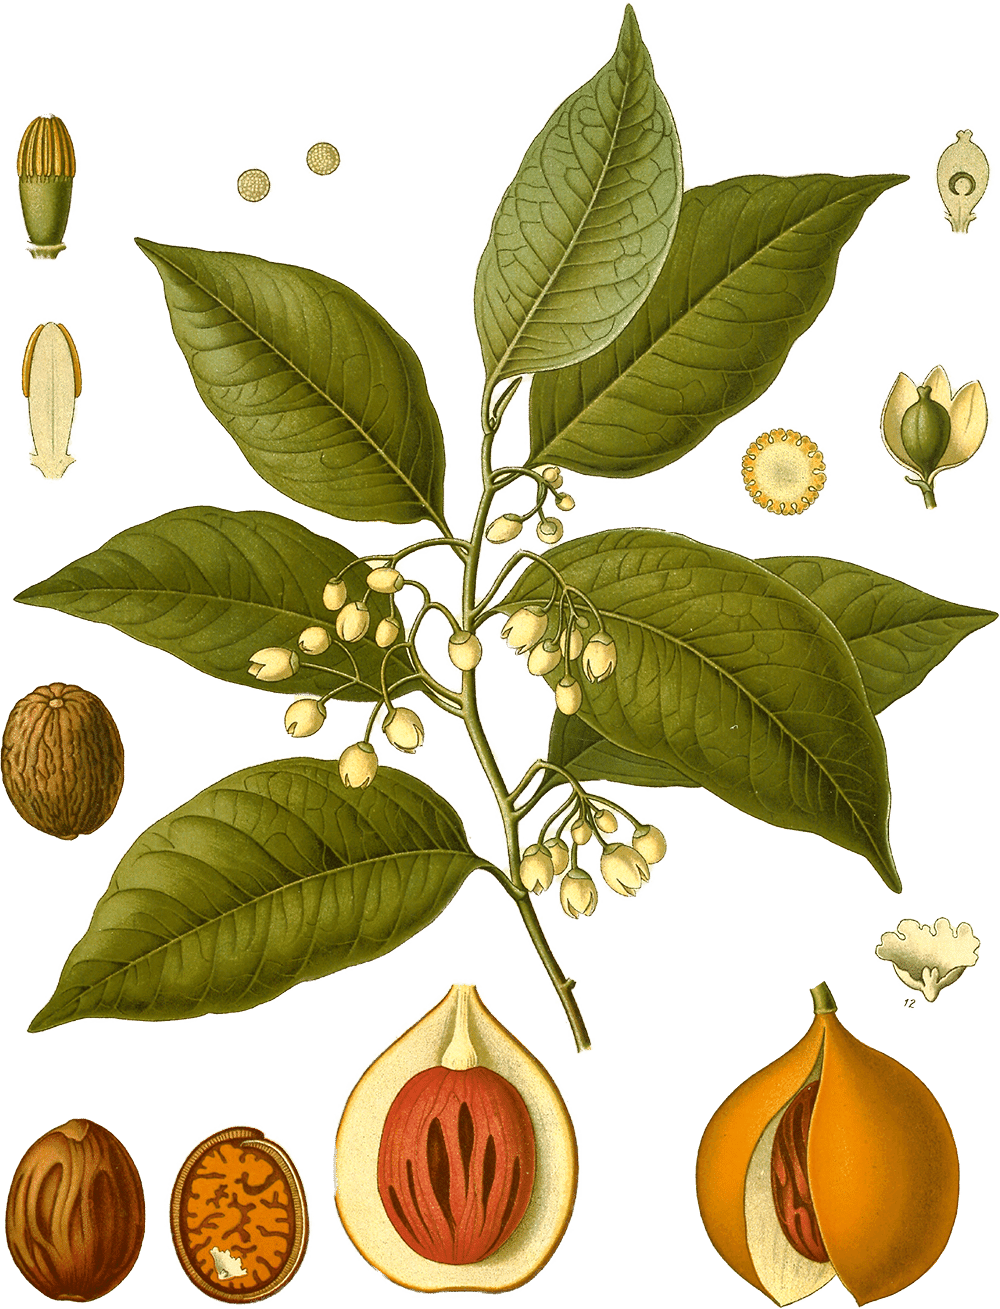
\includegraphics[width=0.45\textwidth]{imgs/nutmeg.png}
    \caption{\textit{Myristica fragrans} in \textit{Köhler's Medizinal Pflanzen} \pvolcite[]{2}[132]{koehler_1887_koehler}}
    \label{fig:nutmeg}
\end{figure}

% \begin{wrapfigure}{r}{0.5\textwidth}
%     \centering
%     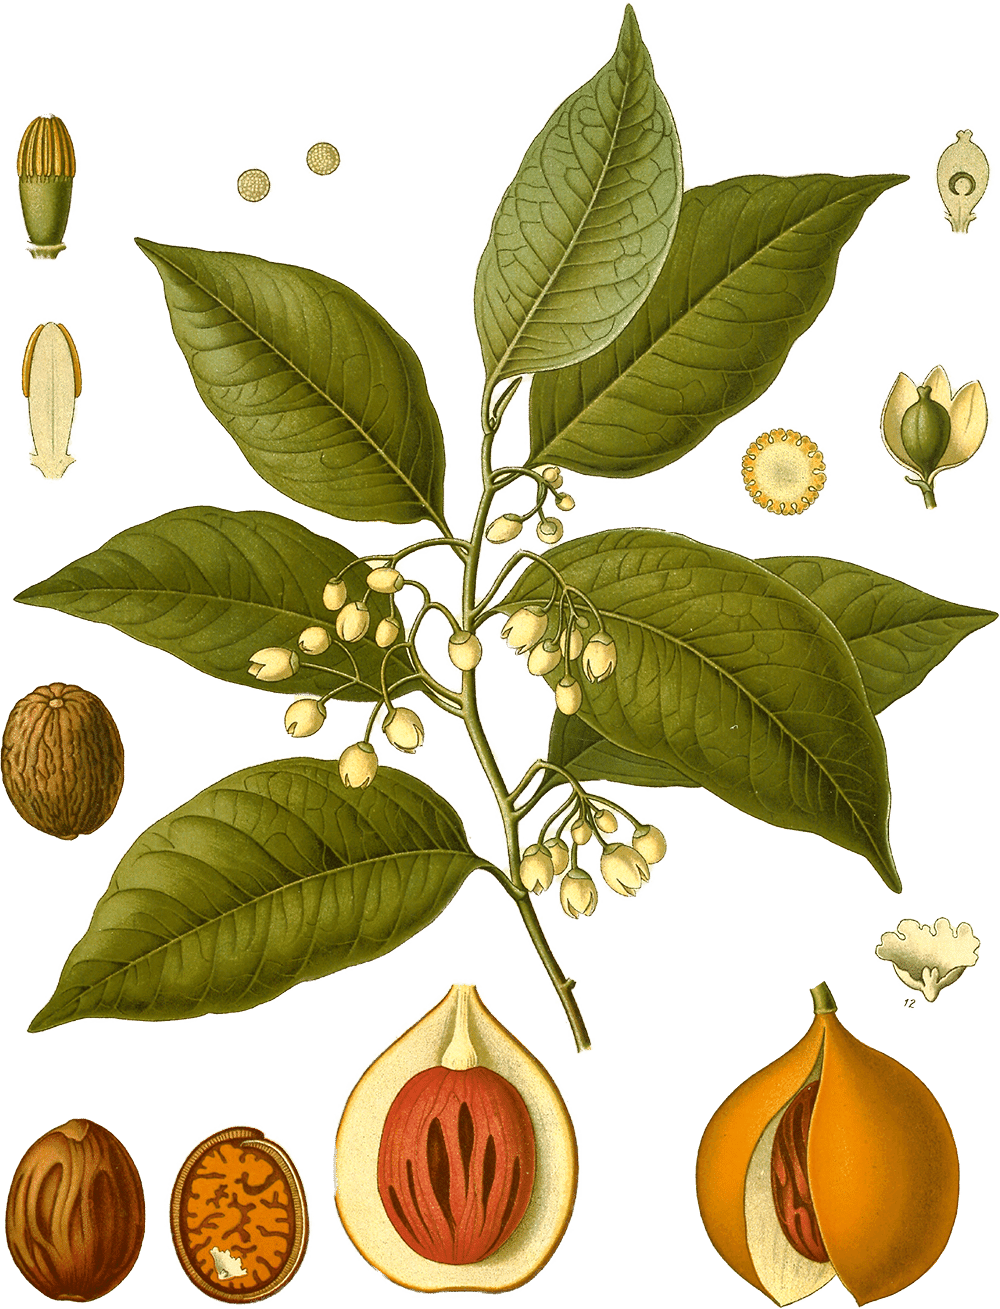
\includegraphics[width=0.5\textwidth]{imgs/nutmeg.png}
%     \caption{\textit{Myristica fragrans} in \textit{Köhler's Medizinal Pflanzen} \pvolcite[]{2}[132]{koehler_1887_koehler}}
%     \label{fig:nutmeg}
% \end{wrapfigure}


\printbibliography

\end{document}
